%%%%%%%%%%%%%%%%%%%%%%%%%%%%%%%%%%%%%%%%%
% Structured General Purpose Assignment
% LaTeX Template
%
% This template has been downloaded from:
% http://www.latextemplates.com
%
% Original author:
% Ted Pavlic (http://www.tedpavlic.com)
%
% Note:
% The \lipsum[#] commands throughout this template generate dummy text
% to fill the template out. These commands should all be removed when 
% writing assignment content.
%
%%%%%%%%%%%%%%%%%%%%%%%%%%%%%%%%%%%%%%%%%

%----------------------------------------------------------------------------------------
% PACKAGES AND OTHER DOCUMENT CONFIGURATIONS
%----------------------------------------------------------------------------------------

\documentclass[12pt]{article}

\usepackage{fancyhdr} % Required for custom headers
\usepackage{lastpage} % Required to determine the last page for the footer
\usepackage{extramarks} % Required for headers and footers
\usepackage{graphicx} % Required to insert images
\usepackage{lipsum} % Used for inserting dummy 'Lorem ipsum' text into the template
\usepackage{wrapfig}
\usepackage{enumitem}

\usepackage[explicit]{titlesec}

\usepackage[export]{adjustbox}

% Margins
\topmargin=0in
\evensidemargin=0in
\oddsidemargin=0in
\textwidth=6.5in
\textheight=9in
\headsep=0.5em 

\linespread{1} % Line spacing

% list spacing
\setlist{nosep}

% caption spacing
\setlength\belowcaptionskip{-5pt}

% \bibliographystyle{plain}

\titleformat{\section}
  {\bfseries}{\thesection}{0em}{#1}
\titlespacing*{\section}{0em}{0em}{0em}[0em]

% Set up the header and footer
\pagestyle{fancy}
\lhead{\AuthorName} % Top left header
\chead{\Title} % Top center header
\rhead{\Subject} % Top right header
\fancyfoot{}
% \lfoot{\lastxmark} % Bottom left footer
% \cfoot{} % Bottom center footer
% \rfoot{Page\ \thepage\ of\ \pageref{LastPage}} % Bottom right footer
\renewcommand\headrulewidth{0.4pt} % Size of the header rule
% \renewcommand\footrulewidth{0.4pt} % Size of the footer rule

\setlength{\parskip}{0.4em}
\setlength\parindent{0pt} % Removes all indentation from paragraphs


\newcommand{\Title}{Project Narrative} % Assignment title
\newcommand{\Subject}{NSTRF 2016}
\newcommand{\AuthorName}{Colin Rennie} % Your name

\begin{document}
\newpage

\begin{center}
{\bf Planning and Control for Tethered Cave Exploration }

\end{center}

%---------------- Introduction ------------------
%Tethered Robot Importance 
%Planetary exploration
%Situations needing tethers for science targets
%Communications

The tether we consider is a spooled, flexible tether which serves two primary purposes: (1) to deploy into and retrieve the exploratory rover from constrained environments with scientific value in terms of mission objectives and (2) for communication between the exploratory and base units.

%---------------- Background ------------------

{\bf Tethered Rover Systems Background \\}
Inspired by the variety of science missions that would be achievable
using a tethered robot but not using a more traditional wheeled rover, 
scientific research in this area has produced substantial progress in 
recent past. This research has focused on several different designs of
tethered robots including notable examples of an eight-legged walking robot attached to a 
stationary base and two-wheeled differential drive pairs of tethered robots. Both designs
feature an actuated winch or spooled tether used for communication and/or 
stability while repelling uneven and difficult terrain.

%Dante II (& lemur II?)
The Dante II robot design consisted of eight legs for locomotion and an 
actuated winch for repelling down steep and difficult terrain. Both actuation 
mechanisms were attached to 
a base frame with a sensor arch protruding from the top of the structure \ref{dante_design}. A variety of
sensing equipment, including a pan/tilt camera and a laser range finder,
 were attached to the arch in order to retrieve and transmit data from remote
 locations. In 1994 the system was deployed into Mount Spurr, an active volcano, 
 in order to record data for further scientific analysis. The robot's control 
 during this time was a combination of supervised autonomous motions and remote
 teleoperation \ref{dante_results}. Aside from a failure where the robot incurred a lateral force at its contact
point with the tether, fell over and was not able to correct itself,
 the 5-day mission was regarded as a success in showing the capabilities of robotic
 systems to act as ``surrogate scientists'', exploring where humans would not otherwise
 be able. 

%Axel platform (+picture)
More recently, NASA's Jet Propulsion Laboratory has been working on a two-wheeled
differential drive tethered robot, appropriately named ``Axel''. The Axel robot 
design features collapsible, paddled wheels, making the system more appropriate for longer 
and more remote missions as this design is more robust to issues such as high-centering and 
failures such as that encountered by Dante II \ref{axel_design}. The tether mechanism is connected to the axel 
between the two wheels and is actively spooled as the wheels move relative to the body of the robot. 
Two variants of the system are presented: one in which Axel is attached to a stationary anchor point, 
and a second where two Axel robots are tethered together and deployed via a central support beam (``DuAxel'') \ref{duaxel}. 

%Motion planning solution
The open question in either design variation is how to plan autonomous descent and corresponding 
ascent paths for the deploying tethered Axel robot in uneven, rocky, extra-planetary terrains. 
A solution framework is presented which projects this complex problem to a two-dimensional plane and, 
building on foundational work addressing the tether constraint problem from a computational geometry 
perspective, extends this work to produce ``controllable'' paths by deriving equations of motion arising from 
the constraints of the Axel robot \ref{axel_planning}. The resulting algorithm first plans the more difficult ascent path and
uses this solution to limit its search for viable descent paths lying in the same homotopy class. 

%Problems
%   Quasi-static, no cable friction with ground assumed
%   solution is planar, over-simplifying the environment
%   assumes static anchor point (base unit)
While this solution represents substantial progress well-grounded in foundational work, the 
assumptions and simplifications made leave much to be desired in terms of robust autonomous
exploration. Projecting these types of difficult terrain environments in two-dimensions and representing
obstacles as simple polygons is a vast simplification of real-world extra-planetary terrains and 
additionally assumes prior and perfect knowledge of the entirety of the environment to be explored. In addition,
the framework assumes frictionless interaction of the tether with the ground plane and quasi-static 
motion of the robot; neither of which will hold in practice. Additionally and perhaps beyond the scope 
of this initial framework, but as this work assumes a static anchor point for the tether an open 
question remains as to how best to plan autonomous motions for the DuAxel configuration where two 
dynamic robots take turns belaying each other.


%---------------- Proposed Research ------------------
{\bf Proposed Research Problems \\}
{\sl The main goal of this research is to address the problem of planning for tethered robots in their 
full workspace, i.e., without directly simplifying the problem to a lower dimension. Doing so will allow 
for kinodynamic, as opposed to quasi-static, solutions. We aim to plan for tethered pairs of robots 
such as the DuAxel configuration as it provides additional freedom and therefore much richer solutions. 
As such, we consider optimization of the constraints of the system (i.e., placement and support of the tether) 
to be a subproblem. Importantly, since we will be operating with imperfect information about the terrain, we also 
desire a coordinated strategy for planning and control which optimizes the amount of time needed to re-plan. }
% TODO: Add online as a goal in presence of imperfect information about the environment

{\bf Problem Description \\}
In this proposal, we consider the DuAxel configuration made up of two tethered Axel robots in a mother-daughter
configuration where the mother is deliberately positioned in a stable position in order to provide support 
to the deploying daughter system. For the sake of this proposal, we make one change to the DuAxel design: 
we imagine that the caster arm which controls the locations of the tether at its connection points on the robots
is actuated in two-dimensions using a ball joint design. The benefits of this design change are explored below. 
We also imagine both robots to be equipped with a means of sensing forces imparted upon them by the tether 
(e.g., force/torque sensors).

{\bf Research Problem 1: Coordinated control of a soft tether \\}
{\sl Goal: Given that the main constraint of our planning problem is the tether itself, we first 
address the subproblem of optimal placement and control of the tether with respect to the planning of 
a coordinated ascent/descent for our tethered pair. }
\begin{wrapfigure}{r}{0.5\textwidth}
  \begin{center}
    \vspace{-0.5in}
    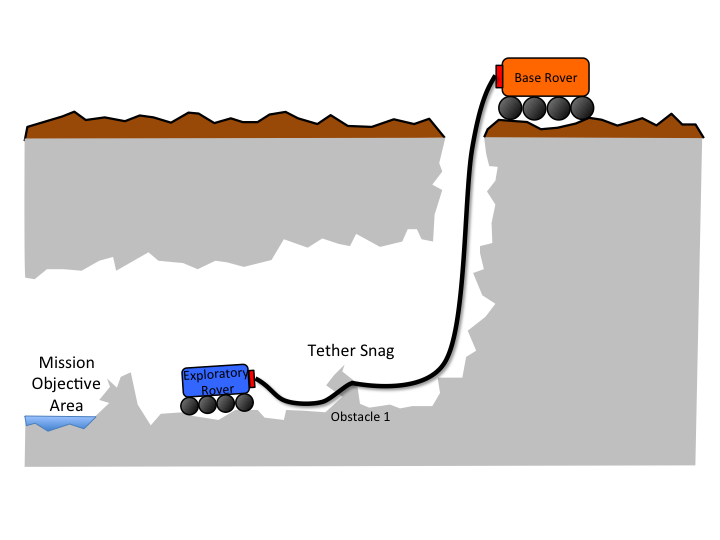
\includegraphics[width=0.48\textwidth, right]{cave_exploration}
  \end{center}
  \vspace{-0.5in}
  \label{fig:cave}
  \caption{A base rover (orange) has deployed an exploratory rover counterpart (blue) into a cave to achieve scientific mission objectives. Pictured, while in route to the mission objective region, the tethered communications cable becomes snagged on an unknown obstacle.}
\end{wrapfigure}
\vspace{-0.15in}

% ONLINE: scaling unforeseen obstacles while executing descents
%     Additionally, this divides our solution homotopy class -- must be integrated with planning
% SNAGGING: high probability of nullifying previously valid solution trajectory


% Outline the problems
In the following, we consider several potentially difficult situations that are likely 
to arise when planning for this system with imperfect information about the terrain. The classic problem 
of an unmodeled obstacle arising during descent is addressed in the planar case in \ref{axel_online}, however beyond 
simply addressing this problem in the full taskspace, we 
desire a solution with two important differences: (1) we desire a re-planning mechanism which exploits 
our control over the tether and (2) we would like to integrate feedback from the re-planning problem 
in our tether control solution to avoiding this new obstacle. A second situation likely to arise as a product 
of friction with the environment is the cable ``snagging'' on small ridges in the terrain. This situation 
has the ability to nullify a previously valid path as it has the potential to severely limit the length 
of available tether and effectively places our tether configuration in a new homotopy class.

% Divide the problems into cases
We can divide the situations as they might arise into two categories: integration (unmodeled obstacle case) 
and avoidance (snagging case). In addressing both cases, we would like to exploit our design choice of an 
actuated ball joint on the caster arm by developing low level control policies able to manipulate the 
configuration of the tether. 

% avoidance case
In the avoidance case, a general solution may be to induce a traveling wave in the tether by employing 
an oscillatory control policy at the actuated caster arm of the Axel robot closest to the tether snag. 
The challenge in this strategy however, is that once the tether is free it's likely to impart a substantial 
force on the robot's counterpart, potentially resulting in dangerous jerking in a partially known environment. 
A potential solution to this problem would be to induce in response a coordinated, counteracting wave from the caster 
arm of the counterpart system. One potential solution would be to build a model (potentially analytically)
of the expected forces on the counterpart robot and design, e.g. a model predictive control-based solution where 
the low-level control policy optimizes its current control with respect to counteracting the incurred force over 
a finite time horizon of future predictions. Conversely, it's possible that taking a model-free approach would 
yield more desirable behavior, in which case we could design a low-level admittance control law, actuating 
the counterpart's caster arm in response to incoming forces from the tether.

% integration case: online re-planning wrt coordination between avoidance control and motion planning algo
In the integration case (encountering an unmodeled obstacle), what we desire in order to not discard current 
progress is a re-planning strategy which gives our motion planner the greatest chance of success in 
our new mapping of the terrain. Because in the most 
difficult integration case the new obstacle effectively divides our solution's homotopy class into two distinct 
new classes, we first want to know whether or not we can surmount this obstacle with the tether (i.e., place the 
tether on either side of the obstacle). Finding the answer to this can be achieved by either casting this as a 
full planning subproblem in task space where the solution will involve reconfiguring the caster arms holding the 
tether such that the tether moves above the obstacle, or by simulating a strategy similar to the avoidance case above. 
If the obstacle is surmountable, this then allows us to plan ascent/descent path pairs in either 
homotopy class independently of one another's class (because we can arbitrarily reconfigure between the two), thus 
removing a substantial constraint on the new motion planning problem.

{\bf Research Problem 2: Kinodynamic motion planning for tethered pairs \\}
{\sl Goal: Complex maneuvers which utilize the full control space of the robot such as those presented above, 
are only possible if we address the planning problem in its full state space. By doing so, we move away from quasi-static 
solutions and are free to take full advantage of additional features of the system, e.g., kinodynamic planning for the mother
robot. }
\begin{wrapfigure}{r}{0.5\textwidth}
  \begin{center}
	\vspace{-0.5in}	
	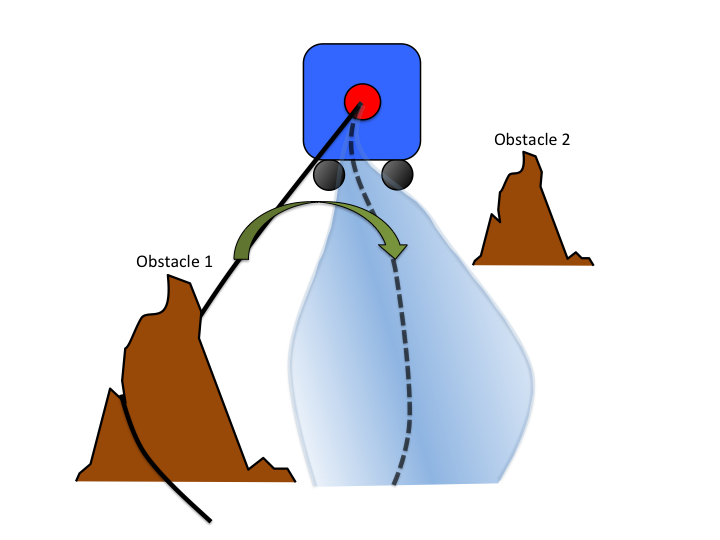
\includegraphics[width=0.48\textwidth, left]{cable_uncertainty}
  \end{center}
  \vspace{-0.5in}
  \label{fig:cable}
  \caption{Employing coordinated control between base and exploratory rovers, we are able to relieve the snagged cable (green arrow) but in doing so are left with uncertainty about where the cable now lies (blue region).}
\end{wrapfigure}
\vspace{-0.15in}

%Problem
For reasons included throughout this proposal, we desire to move away from quasi-static solutions and 
toward solutions which allow us to utilize the robot pair and tether to their full potential toward solving 
these traditionally difficult planning problems. Beyond the added state and control complexities of our 
ball joint caster arm design choice, we additionally would like to plan for both the mother and daughter 
robots simultaneously, which further increases complexity. Doing so, however, allows us to plan much more complex deployments, 
provide dynamic tether stability support to the daughter Axel robot, and reach science targets that we would not otherwise 
be able to reach.

%Solution Sampling-based
Equipped with a model of the cable's dynamics, we have all the tools necessary to address this problem 
using traditional sampling-based motion planning methods, which have been successfully applied to solve similarly 
high dimensional problems \ref{zak_kino}. The typical complaint with these methods, however, is the required time and 
computation required to randomly sample enough points to converge to a solution. Considering that we require 
methods to be able to re-plan in situations such as the above, our desire is to substantially decrease the amount of time 
required to find solutions, while still addressing this problem in its full state space. 

%Solution 
Several techniques can be drawn upon in such a scenario. The first set of approaches involve biasing the sampling of states 
in ways that utilize our in-depth knowledge of the problem we desire to solve. For example, by computing the ``most stable'' support 
position of the mother robot (i.e., perpendicular to the current position of the daughter robot or first encountered wrapped obstacle) 
and biasing in this direction. Additionally worth exploring is whether or not it's effective to solve this problem in 
a 2D projection first, define a broad mapping from 2D space back to the full configuration space, and use this solution to bias samples
in the full space. 

Additionally, it could be possible that by dissecting the problem into multiple subproblem manifolds we can achieve reliable 
solutions much faster than in the full space. This could involve applying machine learning as in \ref{learning_biases}, where the authors 
train a machine learning model to learn the important sub-manifolds of a particular system while also learning which static 
configurations (``biases'') for the static state dimensions would be most effective for solving the current problem. 








% ----------------end of document body---------------------

%---------------- start of references------------------
\newpage
\bibliographystyle{ieeetr}
\small{\bibliography{bibl.bib}}

%---------------- end of references------------------


\end{document}